
\slide{Cenário de experimento}{
\begin{itemize}
    \item Para experimento foram coletados dados de voos regulares do aeroporto de Brasília
    \item Para cada caso de estudo foram treinados 7 agentes.
    \item Cada agente é treinado repetidamente, se aproximando da política gananciosa a cada iteração.
\end{itemize}
}
% >>>>>>>>>>>>>>>>>>
\slide{Cenário de experimento}{
\begin{figure}[]
    \centering
    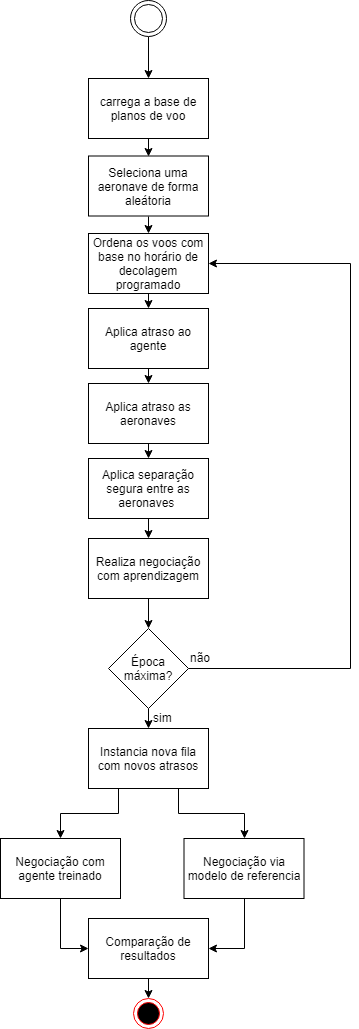
\includegraphics[scale=0.15]{img/experimento.png}
    \caption{Fluxograma de execução do experimento(pag-31)}
    \label{fig:experimento}
\end{figure}
}
\slide{Dados}{
\begin{figure}[H]
    \centering
    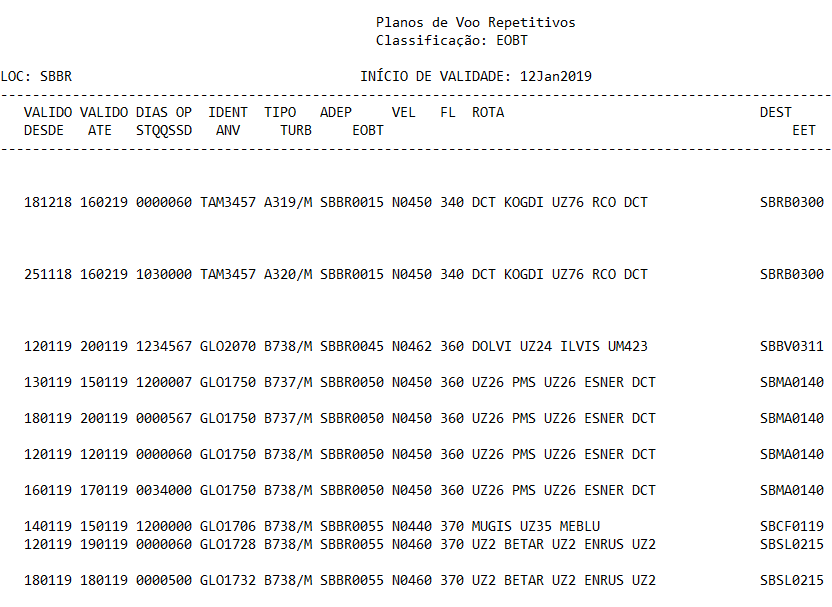
\includegraphics[scale=0.35]{img/exemplo_planodevoo.png}
    \caption{Plano de Voo Regular}
    \label{fig:PlanoVoo}
\end{figure}
}

\slide{Estudos de Caso:}{
\begin{enumerate}
    \item Alocação Homogênea: São desconsiderados os atributos individuais de cada Aeronave. Espera-se que o agente mantenha sua posição na fila sem alterar seu custo. 
    \item Alocação Heterogênea: São consideradas os atributos individuais de cada Aeronave. Espera-se que o agente seja capaz de melhorar seu custo de atraso.
\end{enumerate}
}

% >>>>>>>>>>>>>>>>>>
\slide{Resultados Alocação Homogênea}{
\begin{table}[H]
\centering
\scalebox{0.7}{
\begin{tabular}{|l|l|l|l|l|l|} 
\hline
Aeronaves & Atraso Inicial & Atraso Final~ & Custo Inicial & Custo Final~ & Estados Visitados  \\ 
\hline
TAM3769   & 0              & 0             & 0             & 0            & 0                  \\ 
\hline
TAM3608   & 5              & 5             & 135000        & 337500       & 21                 \\ 
\hline
TAM3074   & 5              & 5             & 135000        & 135000       & 14                   \\ 
\hline
GLO1720   & 10             & 15            & 270000        & 405000       & 15                 \\ 
\hline
ONE6224   & 10             & 10            & 270000        & 270000       & 13                 \\ 
\hline
ONE6233   & 5              & 5             & 135000        & 135000       & 20                 \\
\hline
\end{tabular}}
\caption{Agentes Homogêneos Treinados}
\label{table:case1}
\end{table}}

\slide{Resultado Alocação Homogênea}{
\begin{table}[H]
\scalebox{0.7}{
\begin{tabular}{l|l|l|l|l|l|}
\cline{2-6}
                                 & Aeronave & Atraso Inicial & Atraso Final & Custo Inicial & Custo Final \\ \hline
\multicolumn{1}{|l|}{Antecessor} & ONE6308  & 0              & 0            & 0             & -202500           \\ \hline
\multicolumn{1}{|l|}{Agente}     & TAM3608  & 5              & 5            & 135000             & 337500           \\ \hline
\multicolumn{1}{|l|}{Sucessor}   & ONE6374  & 5              & 5            & 135000             & 135000           \\ \hline
\end{tabular}}
\caption{Aeronave TAM3608 após 25 épocas}
\label{table:tam3608_pos}
\end{table}
 
\begin{table}[H]
\scalebox{0.7}{
\begin{tabular}{l|l|l|l|l|l|}
\cline{2-6}
                                 & Aeronave & Atraso Inicial & Atraso Final & Custo Inicial & Custo Final \\ \hline
\multicolumn{1}{|l|}{Antecessor} & ONE6308  & 0              & 0            & 0             & 0          \\ \hline
\multicolumn{1}{|l|}{Agente}     & TAM3608  & 5              & 5            & 135000             & 135000           \\ \hline
\multicolumn{1}{|l|}{Sucessor}   & ONE6374  & 5              & 5            & 135000             & 135000           \\ \hline
\end{tabular}}
\caption{Aeronave TAM3608 após 100 épocas}
\label{table:tam3608_2}
\end{table}
}

\slide{Resultados Alocação Homogênea}{
\begin{table}[H]
\scalebox{0.7}{
\begin{tabular}{l|l|l|l|l|l|}
\cline{2-6}
                                 & Aeronave & Atraso Inicial & Atraso Final & Custo Inicial & Custo Final \\ \hline
\multicolumn{1}{|l|}{Antecessor} & GLO1829  & 10             & 10           & 270000        & 270000      \\ \hline
\multicolumn{1}{|l|}{Agente}     & GLO1720  & 10             & 15           & 270000        & 405000      \\ \hline
\multicolumn{1}{|l|}{Sucessor}   & GLO1754  & 15             & 10           & 405000        & 270000      \\ \hline
\end{tabular}}
\caption{Aeronave GLO1720 após 25 épocas}
\label{table:pos_glo1720}
\end{table}

\begin{table}[H]
\scalebox{0.7}{
\begin{tabular}{l|l|l|l|l|l|}
\cline{2-6}
                                 & Aeronave & Atraso Inicial & Atraso Final & Custo Inicial & Custo Final \\ \hline
\multicolumn{1}{|l|}{Antecessor} & GLO1829  & 10             & 10           & 270000        & 270000      \\ \hline
\multicolumn{1}{|l|}{Agente}     & GLO1720  & 10             & 10           & 270000        & 270000      \\ \hline
\multicolumn{1}{|l|}{Sucessor}   & GLO1754  & 15             & 15           & 405000        & 405000      \\ \hline
\end{tabular}}
\caption{Aeronave GLO1720 após 100 épocas}
\label{table:glo1720_2}
\end{table}

}
\slide{Alocação Heterogênea}{

\begin{table}[H]
\centering
\scalebox{0.7}{
\begin{tabular}{|l|l|l|l|l|} 
\hline
Aeronaves & Tempo de viagem (Minutos) & Velocidade(Nós) & Relevância & Porte  \\ 
\hline
TAM3769   & 130                       & 450             & 0.925      & M      \\ 
\hline
TAM3608   & 240                       & 450             & 0.925      & M      \\ 
\hline
TAM3074   & 115                       & 450             & 0.925      & M      \\ 
\hline
GLO1720   & 200                       & 440             & 0.835      & M      \\ 
\hline
ONE6224   & 200                       & 450             & 0.634      & M      \\ 
\hline
ONE6233   & 150                       & 450             & 0.634      & M      \\
\hline
\end{tabular}}
\caption{Atributos Aeronaves}
\label{table:atributos}
\end{table}
}

\slide{Resultados Alocação Heterogênea}{
\begin{table}[H]
\centering
\scalebox{0.7}{
\begin{tabular}{|l|l|l|l|l|l|} 
\hline
Aeronaves & Atraso Inicial & Atraso Final & Custo Inicial~ & Custo Final & Estados Visitados  \\ 
\hline
TAM3769   & 0              & 0            & 0              & 0           & 0                  \\ 
\hline
TAM3608   & 5              & 5            & 135000         & 135000      & 20                 \\ 
\hline
TAM3074   & 5              & 5            & 216083         & 216083      & 14                 \\ 
\hline
GLO1720   & 10             & 5            & 264000        & 198005      & 12                 \\ 
\hline
ONE6224   & 10             & 10           & 579255         & 579255      & 13                 \\ 
\hline
ONE6233   & 5              & 5            & 281848         & 281848      & 20                 \\
\hline
\end{tabular}}
\caption{Agentes Heterogêneos Treinados }
\label{table:resultados_hetero}
\end{table}

}




\slide{Resultados dos Agentes}{

\begin{figure}[]
    \centering
    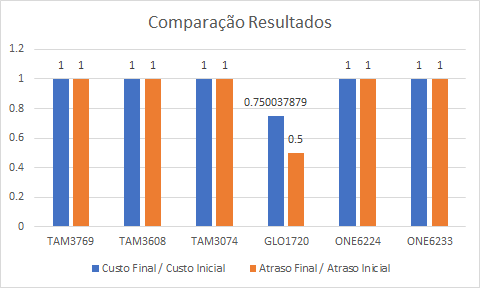
\includegraphics[scale=0.6]{img/compres.png}
    \caption{Comparação dos resultados por agente}
    \label{fig:comp_ag}
\end{figure}
}

\slide{Recompensa na Elaboração de Oferta}{
\begin{figure}[]
    \centering
    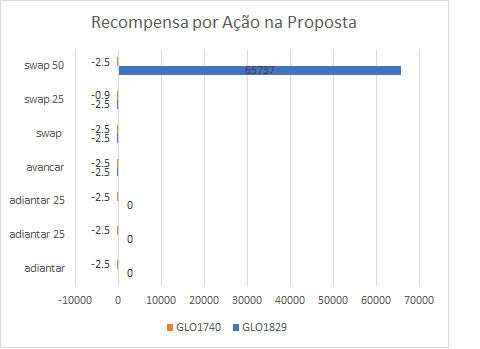
\includegraphics[scale=0.6]{img/recprop.png}
    \caption{Recompensa por Ação nas Propostas aos Antecessores}
    \label{fig:recprop}
\end{figure}
}
\slide{Recompensa na Avaliação de Ofertas}{
\begin{figure}[]
    \centering
    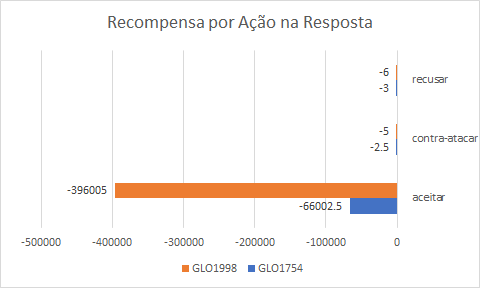
\includegraphics[scale=0.6]{img/recres.png}
    \caption{Recompensa por Ação na resposta ao Sucessores}
    \label{fig:recres}
\end{figure}
}

\slide{Custo das Aeronaves Adjacentes}{
\begin{figure}[H]
    \centering
    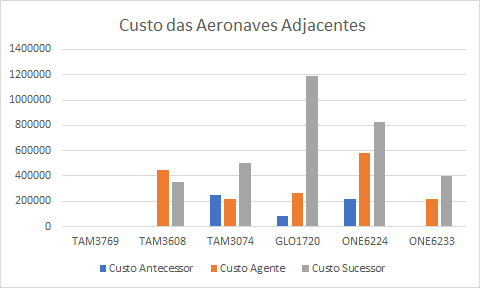
\includegraphics[scale=0.6]{img/custoadj.png}
    \caption{Custo das Aeronaves Adjacentes aos Agentes}
    \label{fig:adj_cost}
\end{figure}
}

\slide{Atributos das Aeronaves Adjactentes}{
\begin{figure}[H]
    \centering
    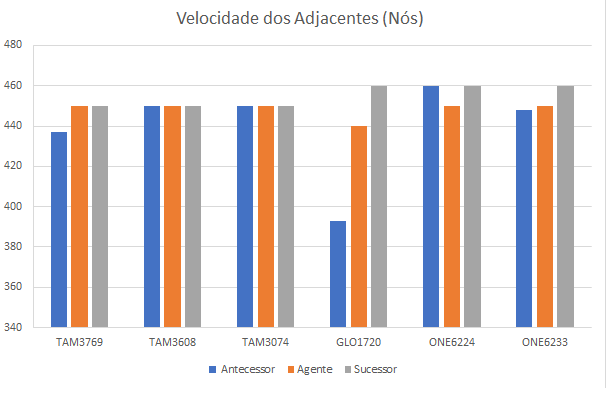
\includegraphics[scale=0.6]{img/VelocidadeAdj.png}
    \caption{Velocidade das Aeronaves Adjacentes}
    \label{fig:adj_vel}
\end{figure}
}
\slide{Atributos das Aeronaves Adjactentes}{
\begin{figure}[H]
    \centering
    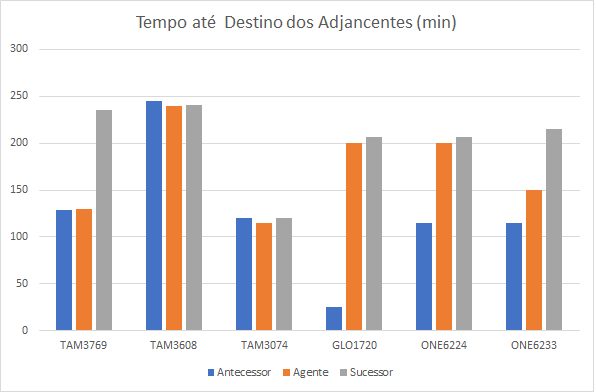
\includegraphics[scale=0.6]{img/tempoadj.png}
    \caption{Tempo até o Destino das Aeronaves Adjacentes}
    \label{fig:adj_time}
\end{figure}
}